\documentclass{book}

\usepackage[all]{nowidow}
\usepackage{graphicx}
\usepackage{xcolor}
\usepackage{sectsty, graphicx, wrapfig}
\usepackage[utf8]{inputenc}
\definecolor{ChapterBlue}{rgb}{0.1,0.6, 0.9}
\chapterfont{\color{ChapterBlue}}  % sets colour of chapters
\sectionfont{\color{cyan}}
\usepackage[font={color=ChapterBlue},figurename=fig.,labelfont={bf}]{caption}

\usepackage{epstopdf}
\usepackage[german]{babel}
\pagestyle{plain}
\title{Design Dokument für TODO}
\author{Christian Stricker \and David Klopp \and Markus Vieth}
\date{\today}

\begin{document}
\frontmatter
\maketitle
\tableofcontents
\mainmatter


\part{Architectural Design}

\chapter{Einleitung}
Im Folgenden werden in diesem Dokument verschiedene Perspektiven des zu entwickelnden Systems betrachtet. Dazu wird das System in Teilsysteme zerlegt und deren Verhalten aufgezeigt.\\
\\
Das System, sowie alle Angaben zum System, beziehen sich dabei auf das "`Requirements Document for TODO"' vom 20. November 2015.
 
\chapter{Externe Sicht}
Das System, als Web-Applikation, interagiert mit anderen Systemen in seiner Umgebung. TODO kommuniziert zur Übertragung von Daten mit mehreren Clients, welche Anfragen senden und Antworten empfangen, und mit weiteren Servern um Daten in den Datenbanken auszutauschen.\\
\begin{figure}[h]
	\vspace{-10pt}
\centering
\includegraphics[width=0.9\linewidth]{Grafik/Diagramm/External}
\caption[Context Diagram]{Context Diagram des Systems im Bezug zu seiner Umgebung}
\label{fig:External}
\end{figure}\\
Die Kommunikation zwischen dem TODO und anderen Servern läuft dabei über das REST-Interface ab. Auch die Clients nutzen REST um Anfragen an das System zu stellen. Die Verbindung wird über HTTPS aufgebaut. Der Nutzer kann zur Kommunikation mit dem System jegliche Software nutzen, welche den Austausch von Daten über HTTPS unterstützt, insbesondere Browser wie Firefox oder Google Chrome. Ein Administrator hat die Möglichkeit über einen Client oder direkt an dem Rechner, auf dem das System läuft, zu arbeiten.

\chapter{Struktursicht}%
\section{Server-Client}
%\documentclass[a4paper,11pt,twoside]{article}
%\usepackage{graphicx}
%\begin{document}

\begin{figure}[h]
	\centering
	\includegraphics[width=0.5\linewidth]{Grafik/Diagramm/Pattern/ClientServer/Kontext.png}
	\caption[]{Client-Server-Modell}
\end{figure}

\subsection*{Client}
Der Client ist der User, der Datensätze, Algorithmen auf den Server hochladen, diese dann dort berechnen lassen und Pakete downloaden kann.

\subsection*{Server}
Der Server bietet dem User den Dienst an, Modelle anhand von schon vorhandenen oder vom User hoch geladenen Datensätzen und Algorithmen zu erstellen. Des Weiteren dient der Server als Datenbank von schon mit verschiedenen Datensätzen erstellten Modellen.\\

\begin{figure}[h]
	\centering
	\includegraphics[width=0.6\linewidth]{Grafik/Diagramm/Pattern/ClientServer/Sequenzdiagramm.png}
	\caption[]{Client-Server-Sequenzdiagramm}
\end{figure}\pagebreak
Der Client versucht eine Verbindung zum Server aufzubauen, der Server versucht ebenfalls bei Anfrage eine Verbindung zum Client Aufzubauen und schickt dem Client eine Bestätigung, das die Verbindung steht. Danach kann der Client Datensätze/Algorithmen hochladen und dem Server eine Anfrage zum Modelle downloaden schicken.

\subsection*{Was spricht für das Client-Server-Modell?}
Das Client-Server-Modell wird verwendet, wenn eine Datenbank oder ein Service von verschiedenen Orten her abgerufen werden soll. Dies ist für beides der Fall. Der User kann global auf den Server zugreifen und Daten hoch und runter laden.\\
Des Weiteren sollen mehrere gleiche Server online sein, damit viele User-anfragen auf mehrere Server verteilt werden können und somit schneller bearbeitet werden können. Der User sieht aber nur den einen Server. Wenn ein Server offline (ausfällt/gewartet)ist und es sind mehrere online, so bekommt der User davon nichts mit und wird auf einen anderen Server geleitet.\\
Nachteile sind:\\
-Die Leistung des Systems ist unberechenbar, wenn die verschiedenen Service im Server-Netzwerk verteilt ist. Dieser Fall existiert in unserem System nicht.\\
-Es gibt Management Probleme, wenn Server in relativ Unabhängigen Besitz ist. Da die Server unabhängig arbeiten und nur zusammenarbeiten, wenn schon vorhandene Modelle/Datensätze auf einem anderen Server angefragt werden, ist dieser Nachteil zu vernachlässigen.





%\end{document}
\section{Microkernel}
Das System stellt seine Funktionalität über die WEKA-Libary zur Verfügung. Damit diese arbeiten kann, werden Algorithmen benötigt. 
Um eine dynamische Ergänzung der Algorithmen zu ermöglichen wird WEKA als Mikrokernel implementiert. 
So können die Algorithmen als interne Server, wenn benötigt, geladen werden und neue Algorithmen können hinzugefügt werden, ohne das der WEKA-Quellcode bearbeitet werden muss. 
Alle Anfragen an WEKA laufen dabei über eine Datenschnittstelle, welche verschiedene Funktionalitäten für den Client bereitstellt.
So kann die Datenschnittstelle zurückgeben, welche Algorithmen von einem bestimmten Datensatz unterstützt werden oder ob ein zu erstellendes Modell bereits in der Datenbank vorhanden ist. 
WEKA übernimmt die Berechnung eines Modells und die Auswertung eines Datensatzes (bzw. eines Algorithmus). 
Der Web-Server übernimmt die Rolle eines Adapters, welcher die REST-Anfragen des Clients auswertet und weitere Instruktionen einleitet.\\
\begin{figure}[h]
\centering
	\vspace{-5pt}
\includegraphics[width=0.7\linewidth]{Grafik/Diagramm/Microkernel}
\caption[Microkernel-Klassen]{Microkernel-Pattern mit WEKA}
\label{fig:Microkernel}
\end{figure}

\subsubsection{Was spricht für den Microkernel?}
Das System soll in der Lage sein stetig mit neuen Algorithmen versorgt zu werden. Das Microkernel-Pattern erlaubt dies, ohne im späteren Verlauf oder gar für jeden Algorithmus den Quellcode verändern zu müssen. Dies erlaubt eine große Flexibilität hinsichtlich der Möglichkeit verschiedene Algorithmen zu verwenden. Ein weiterer Aspekt ist die Trennung von WEKA und den Algorithmen. Dies verringert das negative Beeinflussen beider Parteien untereinander. Des Weiteren erlaubt es ein einfacheres ändern (z.B. Updaten, erweitern der Funktionalität) der Komponenten. In Anbetracht der Vorteile, sind die Performance-Einbußen durch das Pattern nicht weiter relevant.
\section{Reflection}
Um dynamisch später hinzugefügte Algorithmen auch in der Ein- und Ausgabe zu unterstützen, werden die Komponenten "`PluginLoader"' und "`Plugin"' verwendet. Der PluginLoader handhabt die Plugins und erstellt diese falls notwendig. Um dies zu tun, hat der PluginLoader Zugriff auf die Algorithmen. Somit kann der PluginLoader ein Plugin für die Eingabe von Parametern erzeugen, indem er sich von dem entsprechenden Algorithmus die Anzahl der benötigten Parameter ausgeben lässt. Analog kann der PluginLoader ein Plugin zur Ausgabe erzeugen, indem er sich zurückgeben lässt wie die Ausgabedaten aussehen und diese Anhand des gewünschten Ausgabeformats entweder als plain-text, html-text, JSON, PNG-Grafik oder SVG+XML-Grafik aufbereitet.\\

\begin{figure}[h]
\centering
	\vspace{-5pt}
\includegraphics[width=0.7\linewidth]{Grafik/Diagramm/Reflection}
\caption[Reflection-Klasse]{Reflectoin-Pattern mit PluginLoader}
\label{fig:Reflection}
\end{figure}
\subsubsection{Was spricht für Reflection?}
Da das System ständig mit Algorithmen erweiterbar sein soll, wäre es hinderlich, wenn jede Eingabe- und Ausgabemaske für die Algorithmen extra geschrieben werden müssten. Deshalb ist es sinnvoll mithilfe des PluginLoaders diese Masken dynamisch mithilfe der Eingenschaften der Algorithmen zu erzeugen und als Plugins zu speichern. Soll nun das Design der Webseite angepasst werden, eine neue Ausgabe möglich sein oder eine andere Sprache unterstützt werden, so reicht eine Anpassung des PluginLoaders, um passende neue Plugins zu erstellen. Die Permance-Verluste sind an dieser Stelle akzeptabel, da keine Umfangreichen Operationen durchgeführt werden müssen, um den Prozess auszuführen. Auch eine ungewollte Manipulation ist auszuschließen, da der Zugriff auf die Komponenten des System durch den Nutzer sehr stark limitiert ist.


\section{Layer}
Um den Zugriff auf die Datenbank zu beschränken, wird zwischen die Datenschnittstelle und die Datenbank eine Benutzerverwaltung geschaltet. Diese überprüft nun bei jeder Anforderung auf einen Zugriff auf die Datenbank, ob dieser vom aktuellen Nutzer erlaubt ist oder nicht.
\begin{wrapfigure}{l}{0.3\textwidth}
	\vspace{-15pt}
\begin{center}
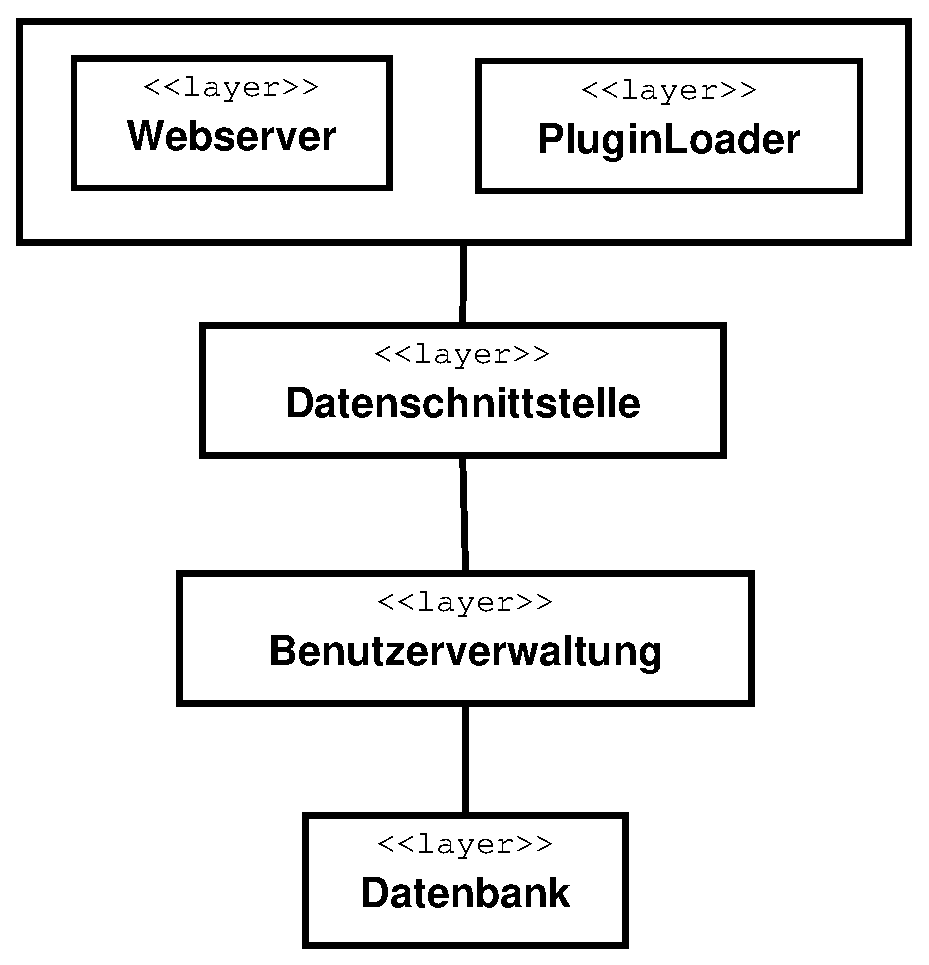
\includegraphics[width=1\linewidth]{Grafik/Diagramm/Layer}
\end{center}
\vspace{-15pt}
\caption[Layer-Klassen]{Layer-Pattern mit Benutzerverwaltung}
\label{fig:Layer}
\vspace{-35pt}
\end{wrapfigure}\\
\\
Das Layer-Pattern hilft einen unerlaubten Zugriff auf die Datenbank zu verhindern und stellt sicher, dass jeder zugriff erst über die Benutzerverwaltung erlaubt wird. Ein weiterer Vorteil stellt die Flexibilität der einzelnen Schichten dar, so kann die Datenschnittstelle statt der lokalen Datenbank auch die Datenbank eines anderen Servers über REST abgerufen, da die Kommunikationswege innerhalb des Layer-Pattern identisch sind.
\\
\section{Blackboard}
\subsubsection{Was spricht gegen Blackboard?}
Das hauptsächliche Einsatzgebiet des Blackboard-Patterns besteht darin, komplexe Sachverhalte auf kleinere Teilprobleme zu reduzieren und diese von sogenannten Experten lösen zu lassen. Anschließend wird das Gesamtergebnis aus den einzelnen Teilergebnissen zusammengesetzt. 
Unser System hingegen hat einen klar definierten sequenziellen Programmablauf: \\
- Benutzereingabe\\
- Auswertung der Eingabe\\
- Datenbankzugriff oder Berechnung.\\
Es macht daher keinen Sinn, Teilprobleme bilden zu wollen. Bei der spezifischen Implementierung eines Algorithmus könnte dieses Pattern eventuell Anwendung finden.



\section{Broker}
\subsubsection{Was spricht gegen Broker-Modell?}
Das Broker-Modell vermindert die Performance, da alle Komponente des Systems nur indirekt angesprochen werden. Des Weiteren hängt die Kommunikation der einzelnen Systeme von vielen Komponenten ab und ist deshalb Fehleranfällig.
Sinnvoll wäre der Broker nur, wenn viele verschiedene Clients auf viele verschiedenen Server auf viele verschiedene Service zugreifen wollen. Die Anzahl der Services unseres Servers ist sehr überschaubar und deshalb ist der Broker zu ineffizient für unseren Server.
\section{MVC}
\documentclass{book}

\usepackage{graphicx}
\usepackage{xcolor}
\usepackage{sectsty}
\definecolor{ChapterBlue}{rgb}{0.1,0.6, 0.9}
\chapterfont{\color{ChapterBlue}}  % sets colour of chapters
\sectionfont{\color{cyan}}


\usepackage[german]{babel}
\pagestyle{plain}
\title{Design Document}
\author{Christian Stricker \and David Klopp \and Markus Vieth}
\date{\today}

\begin{document}


Um zu verstehen wie die Interaktion zwischen Nutzer und System funktioniert, ist es notwendig die Kommunikation der einzelnen Komponenten, die zuständig zum Generieren des UI sind, näher zu beleuchten. 
Besonders geeignet hierfür ist das Model-View-Controller (MVC) Pattern. 
Im folgenden wird zunächst genauer auf die Erzeugen der UI, in unserem Fall eine Website, und anschließend auf die Einbindung einzelner Darstellungskomponenten in dieses eingegangen. \\

\begin{center}
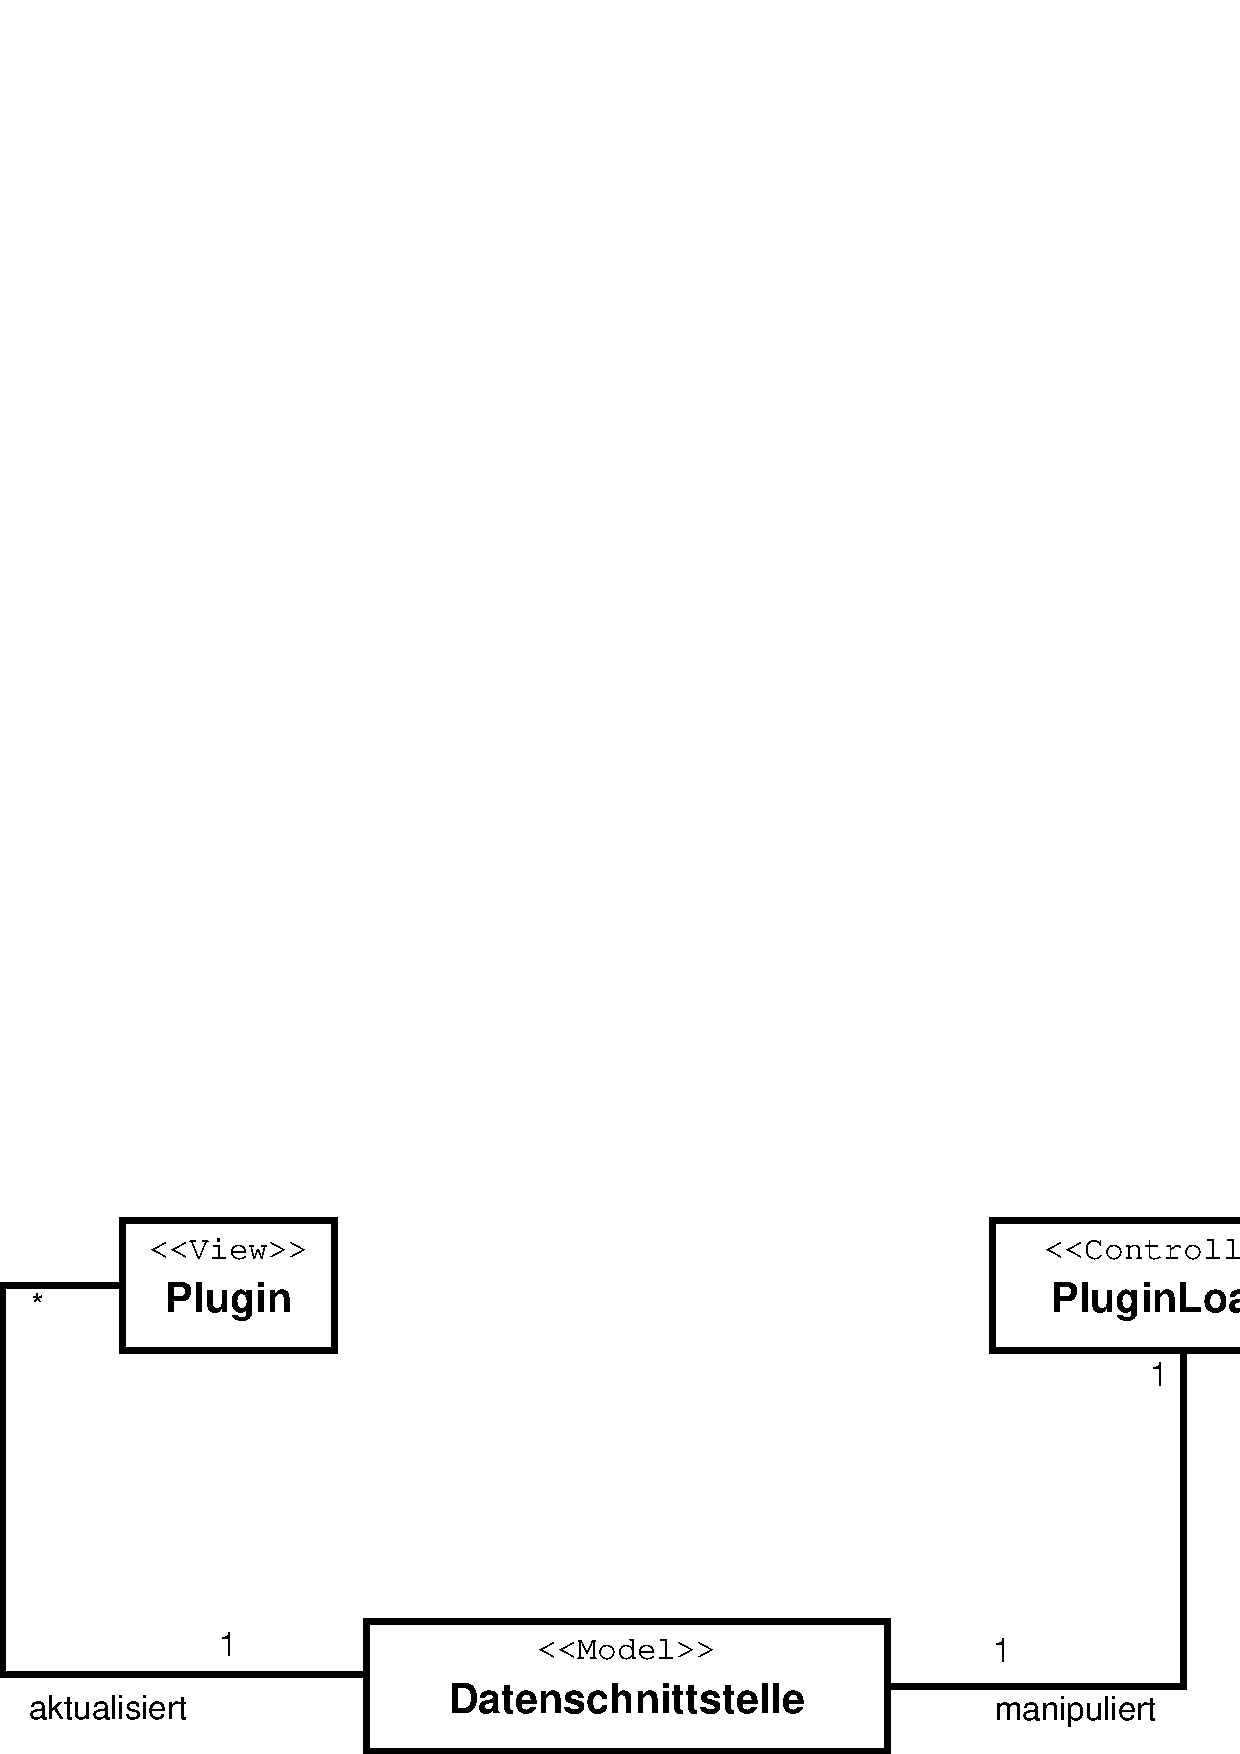
\includegraphics[scale=0.6]{../Grafik/Diagramm/Pattern/MVC/Website/Kontextdiagramm.png}
\end{center}

Die Website ist der für den Benutzer sichtbare Teil des Systems. Betätigt der Nutzer auf dieser Seite eine Schaltfläche, so werden seine Eingaben durch den Webserver ausgewertet und an die entsprechenden Instanzen im System weitergeleitet. Sollen in etwa benutzerbezogene Daten abgefragt werden, so greift der Webserver auf die Datenschnittstelle zu, die die entsprechenden Daten über eine SPARQL Anfragen an die RDF-Datenbank bereitstellt. Auf Basis dieser Rückgabe generiert der Webserver nun die entsprechende Website und  zeigt sie dem Nutzer an.
Sollten sich die Daten in der Datenbank ändern, so registriert die Datenschnittstelle dies und informiert die Website entsprechend, damit die Anzeige geupdated werden kann.

\begin{center}
\includegraphics[width=1.0\linewidth]{../Grafik/Diagramm/Pattern/MVC/Website/Sequenzdiagramm.png}
\end{center}

\end{document}
\section{Pipe and Filter}
\subsubsection{Was spricht gegen Pipe-and-Filter-Pattern?}
Der große Vorteil des Pipe-and-Filter-Pattern besteht darin kontinuierliche Datenströme, mit Hilfe verschiedener Filterbausteine, asynchron und meist unabhängig von einander zu verarbeiten. Da das System allerdings hauptsächlich auf einfachen Dateiaustausch und kurze Anfragen an den Server basiert, reicht es vollkommen aus eine normale https Verbindung zu verwenden ohne eigene Filterströme zwischenzuschalten. Dieses Pattern wäre für die Kommunikation zwischen Client und Server zu mächtig und würde lediglich zu unnötigen Leistungseinbußen führen.%
 
\chapter{Interaktionssicht}
\section{} %weiß ich nicht genau ob die notwendig ist, da sie aber bei srtructuralLayer ist wäre es so einheitlich
\subsection{Login}
\begin{figure}[h]
	%\centering
	\hspace{-0.25\linewidth}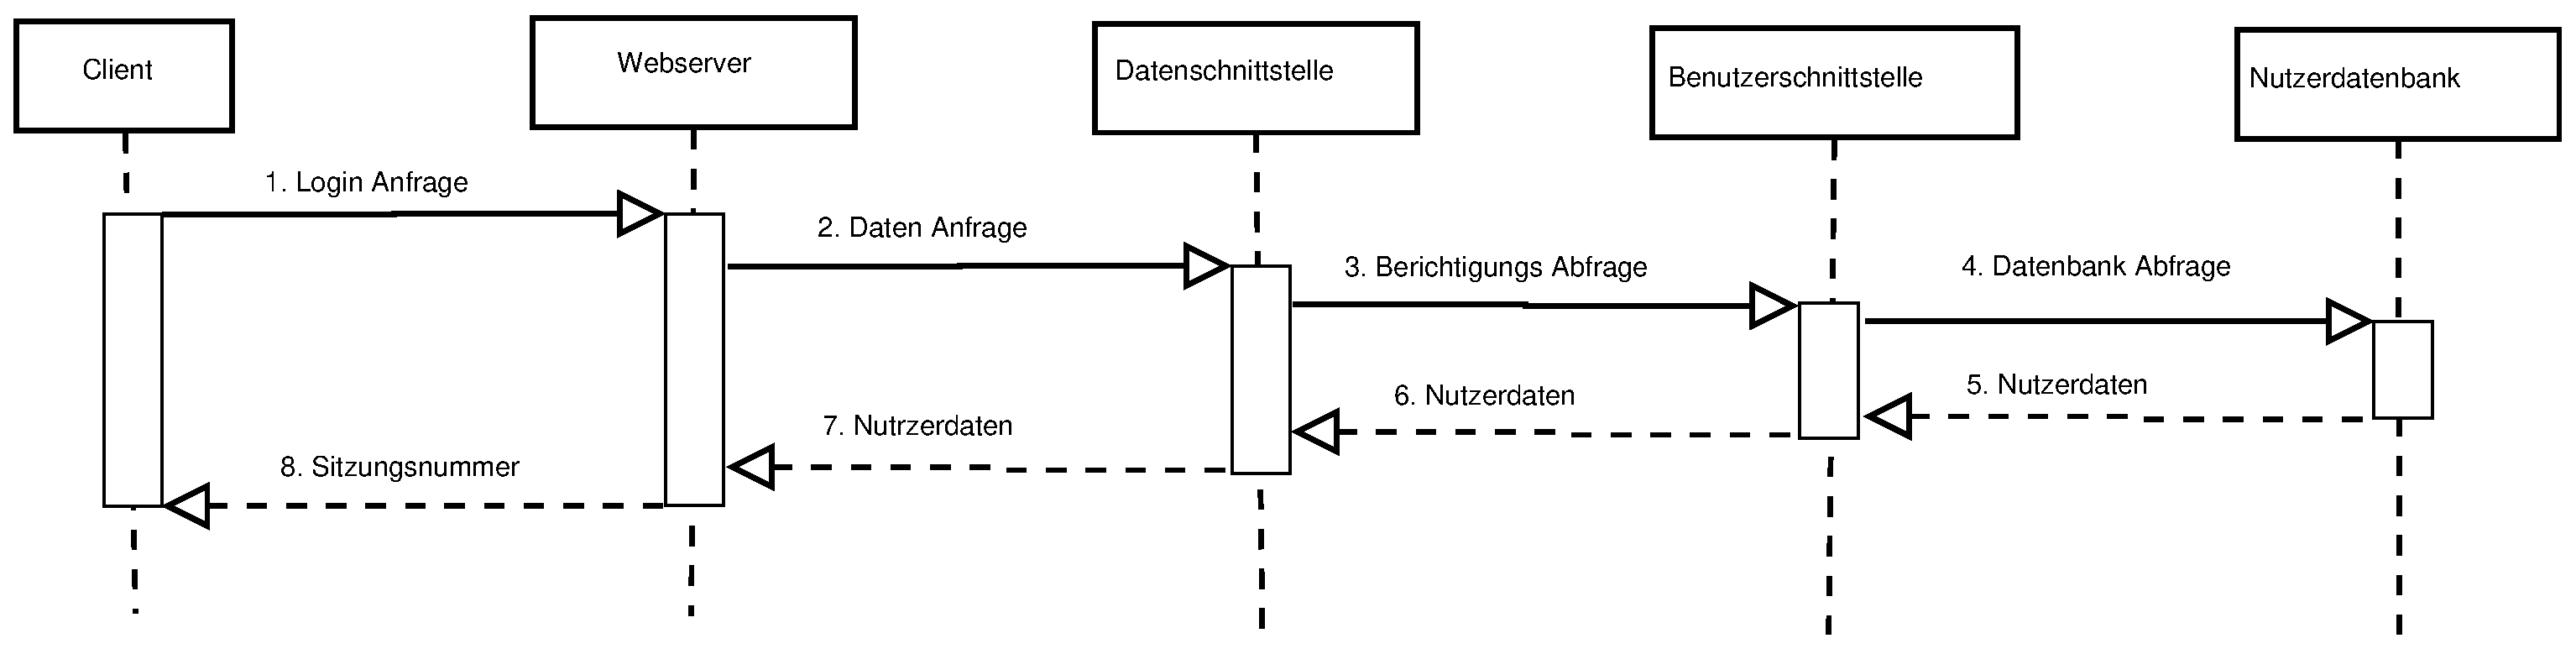
\includegraphics[width=1.5\linewidth]{Grafik/Diagramm/Szenarios/Login}
	\caption[]{Anmeldung eines Benutzers}
\end{figure}

\noindent Nachdem der Benutzer die Startseite aufgerufen hat, kann er sich über ein Formular auf der Seite anmelden. Nach dem Klick auf die entsprechende Schaltfläche wird eine Login Anfrage an den Webserver geschickt. Dieser beauftragt die Datenschnittstelle die erforderlichen Nutzerdaten abzufragen. Hierzu wird die Benutzerschnittstelle angesprochen, die prüft, ob es sich bei den Anmeldedaten um einen registrierten und zugangsberechtigten Nutzer handelt. Sollte dies der Fall sein, so werden die angeforderten Daten aus der Nutzerdatenbank ausgelesen und in der selben Hierarchie bis zum Webserver nach oben gereicht. Dort angelangt wird dem Nutzer eine Sitzungsnummer zugewiesen und ihm zu Zugang zu seinem Account gewährt. 

\subsection{Algorithmus hinzufügen}
\begin{figure}[h]
	%\centering
	\hspace{-0.25\linewidth}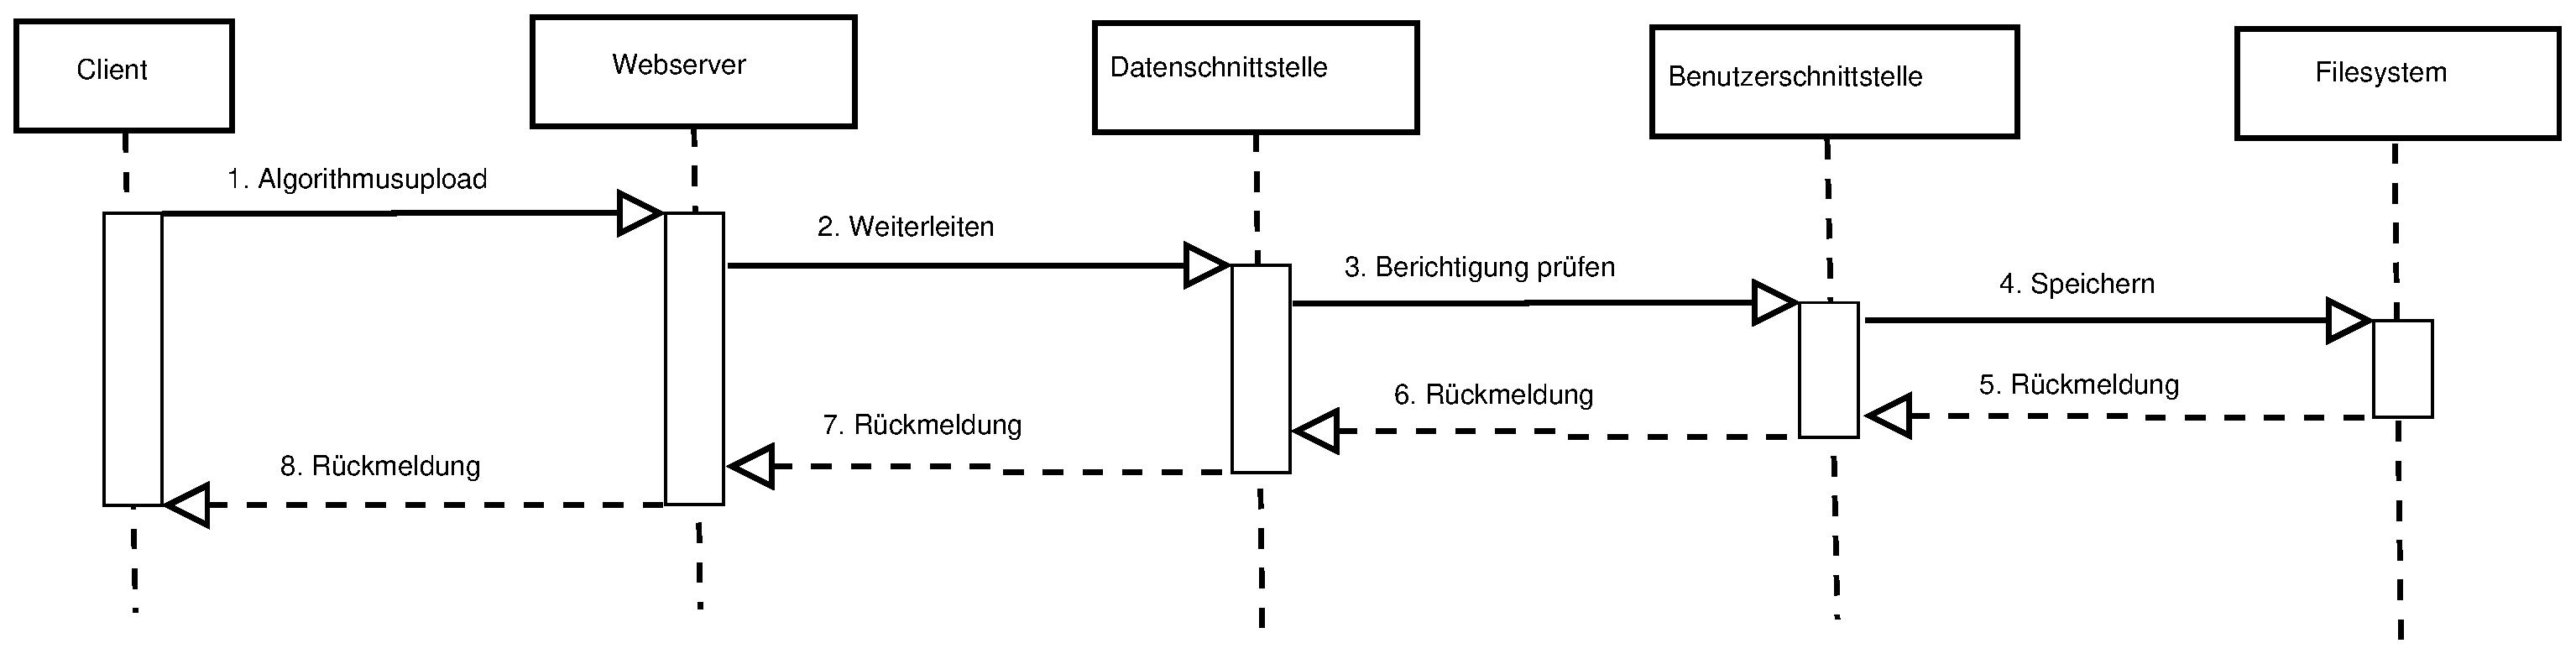
\includegraphics[width=1.5\linewidth]{Grafik/Diagramm/Szenarios/Algorithmus}
	\caption[]{Upload eines Algorithmus}
\end{figure}

\noindent Der Nutzer schickt eine Anfrage zum Upload eines Algorithmus an den Webserver. Dieser delegiert die Nachfrage an die Datenschnittstelle, die diese ihrerseits an die Benutzerschnittstelle zustellt. Dort wird geprüft ob der Nutzer eine Berechtigung zum Upload eines Algorithmus hat, sprich ob er auf dem System registriert ist oder nicht. Sollte er die erforderlichen Kriterien erfüllen, so wird dem Admin der Algorithmus per E-Mail zugestellt und der Benutzer wird über die erfolgreiche Zustellung informiert. Nach Prüfung der übermittelten Daten kann der Admin diese in das Filesystem des Systems integrieren.
\chapter{Anhang}
\begin{figure}[h]
%\centering
%\vspace{-130pt}
\hspace{-0.15\linewidth}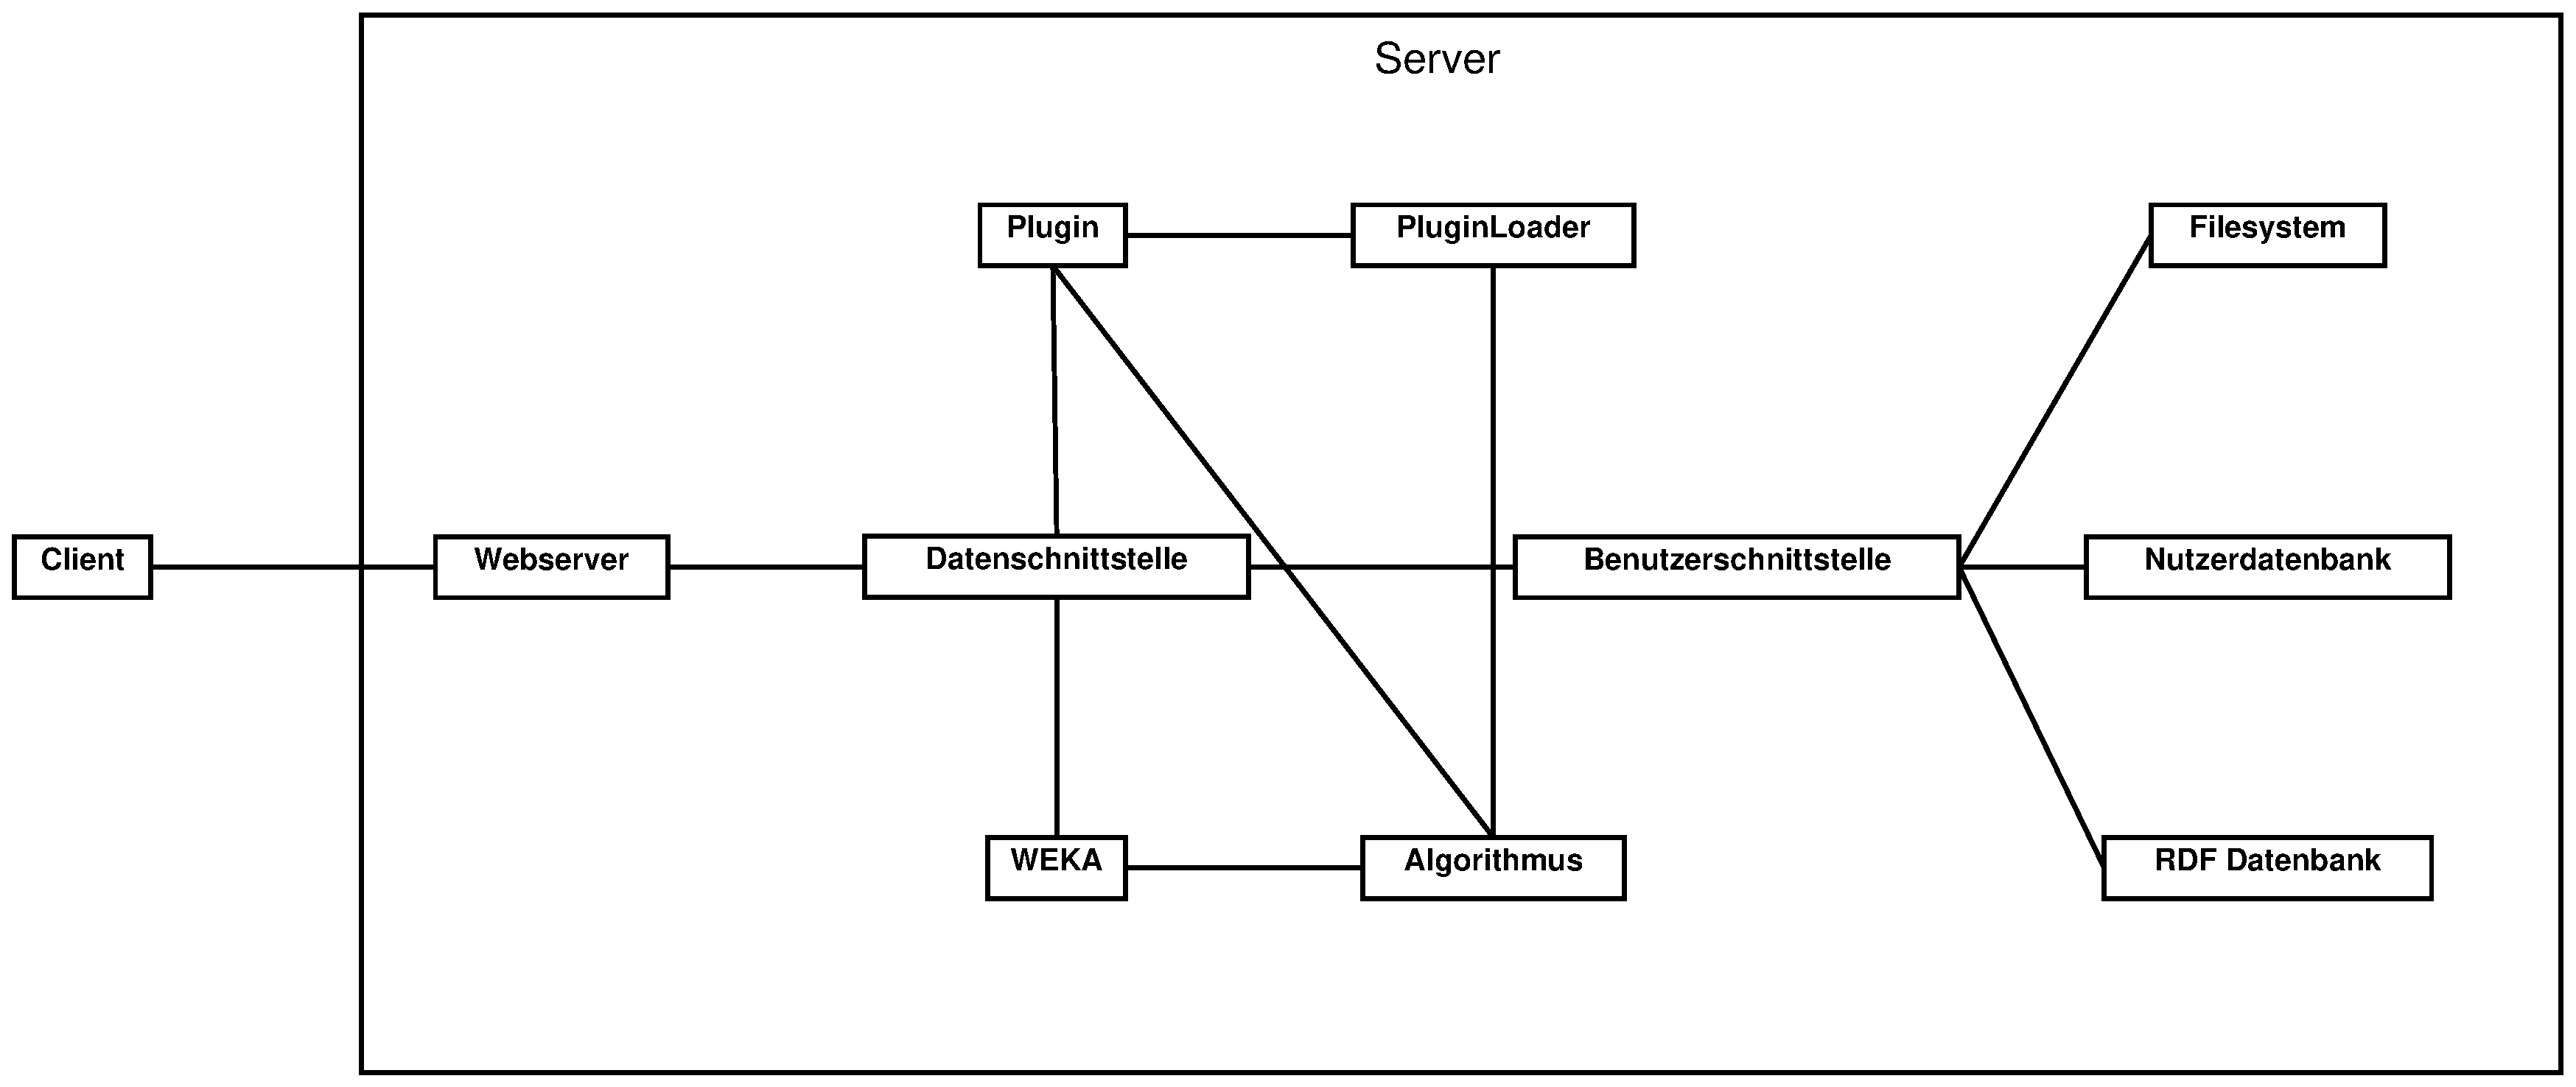
\includegraphics[width=1.5\linewidth]{Grafik/Diagramm/Gesamt}
\caption[Gesamtsystem]{Skizze der Verhältnisse im gesamten System}
\label{fig:Gesamt}
\end{figure}

 
\end{document}

%%% Local Variables:
%%% mode: latex
%%% TeX-master: t
%%% End